%template1.tex
%The following LaTeX source file represents the simplest kind of slide presentation; no overlays, no included graphics. Substitute your favorite style for ``pascal''. To create the PDF file template1.pdf, (1) be sure to use the prosper class, then (2) execute the command latex template1.tex, and (3) the command dvipdf template1.dvi.

%%%%%%%%%%%%%%%%%%%%%%%%%%%%%%% template1.tex %%%%%%%%%%%%%%%%%%%%%%%%%%%%%%%%%%%
\documentclass[a4paper,blends,pdf,colorBG,slideColor]{prosper}
% definitions for slides for CSC544
% Lutz Hamel, (c) 2007

\hypersetup{pdfpagemode=FullScreen}

\usepackage{times}
\usepackage{latexsym}
\usepackage{alltt}
\usepackage{booktabs}
\usepackage{amsmath}
\usepackage{amsopn}
\usepackage{amsfonts}
\usepackage{amssymb}
%\usepackage[usenames]{color}

\def\sign{\qopname\relax{no}{sign}}
\def\argmax{\qopname\relax{no}{argmax}}
\def\argmin{\qopname\relax{no}{argmin}}

\newcommand{\grad}{\ensuremath{\nabla}} 
\newcommand{\loss}{\ensuremath{{\cal L}}}
\newcommand{\err}{\mbox{err}}
\newcommand{\mse}{\mbox{mse}}
\newcommand{\acc}{\mbox{acc}}
\newcommand{\Integer}{\ensuremath{\mathbb{N}}}
\newcommand{\size}[1]{{|{#1}|}}
\newcommand{\Rnspace}[1]{\ensuremath{\mathbb{R}^{#1}}}
\newcommand{\Real}{\ensuremath{\mathbb{R}}}
\newcommand{\mytt}[1]{{\small\tt{#1}}}
\newcommand{\textemph}[1]{{\em #1}}
\newcommand{\suchthat}{\mid}
\newcommand{\orbar}{\;|\;}
\newcommand{\bs}[1]{\begin{slide}{#1}\ptsize{8}}
\newcommand{\es}{\end{slide}}
\newcommand{\co}{\,\colon\;}
\newcommand{\pair}[2]{\ensuremath{( {#1}, {#2} )}}
\newcommand{\model}[1]{\hat{#1}}
\newcommand{\ul}[1]{{\bf\em #1}}
\newcommand{\ol}{\overline}
\newcommand{\definition}[1]{{\bf Definition: }{\em #1}}
\newcommand{\example}[1]{{\bf Example: }{#1}}
\newcommand{\abs}[1]{|{#1}|}
\newcommand{\mytab}{\makebox[.1in]{}}

\newcommand{\fdef}[1]{
\begin{center}
\fbox{
\begin{minipage}{3.5in}
{\bf Definition:}
{#1}
\end{minipage}
}
\end{center}
}

\newcommand{\fframe}[1]{
\begin{center}
\fbox{
\begin{minipage}{3.5in}
{#1}
\end{minipage}
}
\end{center}
}

\newcommand{\nframe}[1]{
\begin{center}
\begin{minipage}{3.5in}
{#1}
\end{minipage}
\end{center}
}

\newenvironment{Rcode}
	{
		\scriptsize
		\begin{quote}
		\begin{alltt}
	}
	{
		\end{alltt}
		\end{quote}
	}




\begin{document}

\bs{$\nu$-SVMs}
In the traditional softmargin classification SVM formulation we have a
penalty constant $C$ such that
\[
C \propto \frac{1}{\mbox{size of margin}}.
\]
Furthermore, there is no {\em a priori} guidance as to what $C$ should be set to - the default
is a value of 1. However, the precise value needs to be determined experimentally.

\es


\bs{$\nu$-SVMs}

Sch\"{o}lkopf {\em et al.} suggest an alternative formulation of {\bf\em softmargin SVMs based
on the $\nu$ parameter}\footnote{B. Sch\"{o}lkopf, A. Smola, R. C. Williamson, and P. L. Bartlett. {\em New Support Vector Algorithms.} Neural Computation, 12:1207�1245, 2000.} with $\nu\in [0,1]$.

The advantages of the {\bf\em $\nu$ parameter} formulation are that it represents an {\bf \em upper bound
on the fraction of number of margin errors} allowed,
\begin{eqnarray*}
\nu = .1 &\rightarrow & \mbox{a max. of 10\% of training set can be margin errors}\\
\nu = .8 &\rightarrow & \mbox{a max. of 80\% of training can be margin errors}
\end{eqnarray*}
and that it is proportional to the size of the margin,
\[
\nu \propto \mbox{size of margin}
\]

This implies that determining a value for $\nu$ is a more intuitive process that finding a value for the penalty constant $C$.
\vspace{.2in}
\es

\bs{$\nu$-SVC}
{\small
We can formulate the $\nu$-SVC\footnote{$\nu$-SVC means $\nu$ support vector classification.} problem in the primal version as follows,
\[
\min_{\ol{w},\ol{\xi},\rho,b} \phi(\ol{w},\ol{\xi},\rho) = \frac{1}{2}\ol{w}\bullet\ol{w} - {\color{red}\nu\rho} + \frac{1}{l}\sum_{i=1}^l \xi_i
\]
\[
\begin{array}{rl}
\mbox{subject to} & y_i(\ol{w}\bullet\ol{x}_i - b) \ge {\color{red}\rho} -\xi_i\\
& \xi_i \ge 0\\
& \rho \ge 0
\end{array}
\]
Here $\ol{\xi}$ represents the set of slack variables as before.

{\bf Observations:} 
\begin{itemize}
\item We no longer have a constant margin of value 1, instead we consider the size of the margin an explicit optimization variable - $\rho$.
\item Observe that if $\ol{\xi} = \ol{0}$ then the margin is $2\rho/\ol{w}\bullet\ol{w}$.
\item We don't directly penalize the size of the margin errors, instead we penalize the size of the margin - term $\nu\rho$.
\end{itemize}
}
\es

\bs{Dual $\nu$-SVC}
\small
The Lagrangian,
\begin{align*}
L(\ol{\alpha},\ol{\beta},\delta,\ol{w},\ol{\xi},\rho,b) &=  \frac{1}{2}\ol{w}\bullet\ol{w} - \nu\rho + \frac{1}{l}\sum_{i=1}^l \xi_i\\
&\quad - \sum_{i=1}^l \alpha_i(y_i(\ol{w}\bullet\ol{x}_i - b) - \rho + \xi_i)\\
&\quad - \sum_{i=1}^l \beta_i \xi_i\\
&\quad - \delta\rho
\end{align*}
with $\ol{\alpha}_i, \ol{\beta}_i, \delta \ge 0$.

Where the optimization problem is
\[
\max_{\ol{\alpha},\ol{\beta},\delta} 
\min_{\ol{w},\ol{\xi},\rho,b} 
L(\ol{\alpha},\ol{\beta},\delta,\ol{w},\ol{\xi},\rho,b).
\]
\es

\bs{KKT Conditions}
\small
A solution $\ol{\alpha}^*, \ol{\beta}^*,\delta^*,\ol{w}^*,\ol{\xi}^*, b^*$, and $\rho^*$ has to satisfy the KKT conditions,
\begin{align*}
\frac{\partial L}{\partial \ol{w}}(\ol{\alpha},\ol{\beta},\delta, \ol{w}^*,\ol{\xi},\rho,b) &= 0,\\
\frac{\partial L}{\partial \xi_i}(\ol{\alpha},\ol{\beta},\delta,\ol{w},\xi^*_i,\rho,b) &= 0,\\
\frac{\partial L}{\partial \rho}(\ol{\alpha},\ol{\beta},\delta,\ol{w},\ol{\xi},\rho^*,b) &= 0,\\
\frac{\partial L}{\partial b}(\ol{\alpha},\ol{\beta},\delta,\ol{w},\ol{\xi},\rho,b^*) &= 0,\\
\alpha^*_i (y_i(\ol{w}^*\bullet\ol{x}_i - b^*) + \xi^*_i -\rho^*)&= 0, \\
\beta^*_i\xi^*_i&= 0,\\
\delta^*\rho^*&= 0,\\
y_i(\ol{w}^*\bullet\ol{x}_i - b^*) + \xi^*_i -\rho^*&\ge 0, \\
\alpha^*_i &\ge 0,\\
\beta^*_i &\ge 0,\\
\delta^*&\ge 0,\\
\xi^*_i &\ge 0,
\end{align*}
for $i = 1,\ldots,l$.
\es

\bs{Dual $\nu$-SVC}
\small
Taking the partial derivatives of $L(\ol{\alpha},\ol{\beta},\delta,\ol{w},\ol{\xi},\rho,b)$ with respect to the primal variables and setting them to $0$ we obtain,

\begin{gather*}
\ol{w} = \sum_{i=1}^l \alpha_i y_i\ol{x}_i\\
\alpha_i + \beta_i = \frac{1}{l}\\
\sum_{i=1}^{l}\alpha_i y_i = 0\\
{\color{red}\sum_{i=1}^l \alpha_i = \nu+ \delta}
\end{gather*}

Plugging these back into the Lagrangian gives us our dual optimization problem.
\es

\bs{Dual $\nu$-SVC}
\small

This gives us the a training algorithm for softmargin $\nu$-SVC with the kernel $k(\ol{x}_i,\ol{x}_j)$ substituted
for the dot product in input space,
\fframe{
\[
\max_{\ol{\alpha}}  \phi'(\ol{\alpha}) = 
  \max_{\ol{\alpha}} \left ( - 
  \frac{1}{2}\sum_{i=1}^l \sum_{j=1}^l y_i y_j \alpha_i \alpha_j k(\ol{x}_i,\ol{x}_j)\right )
\]
subject to the constraints,
\begin{eqnarray*}
&&\sum_{i=1}^l y_i \alpha_i = 0 \\
&&\sum_{i=1}^l \alpha_i \ge \nu \\
&&1/l \ge \alpha_i  \ge 0,  i = 1,\ldots,l
\end{eqnarray*}
}
Compared to the dual optimization problem of C-SVCs we have two differences: (a) we lost the term
$\Sigma \alpha_i$ in the objective function and (b) we have an additional constraint due to $\rho$.
\es

\bs{Dual $\nu$-SVC}
Turns out that our decision function stays the same as in the $C$ classifiers,
\fframe{
\[
\model{f}(\ol{x}) = \sign \left ( \sum_{i = 1}^l \alpha^*_i y_i k(\ol{x}_i, \ol{x}) - b^* \right ).
\]
}

Here, as before, $b^*$ can be computed from support vectors that are not bound, $0 < \alpha_i < 1/l$.
\es


\bs{$\nu$-SVC}
\begin{center}
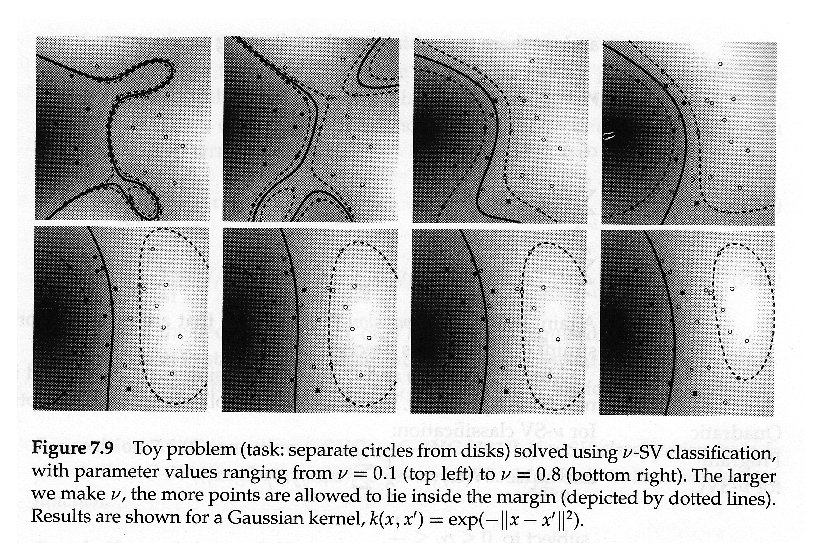
\includegraphics[height=60mm]{images/nu-svc-fig.eps}
\end{center}
{\footnotesize (source: "Learning with Kernels", Sch\"olkopf and Smola, MIT, 2002) }
\es

\bs{$\nu$-SVC}
\begin{center}
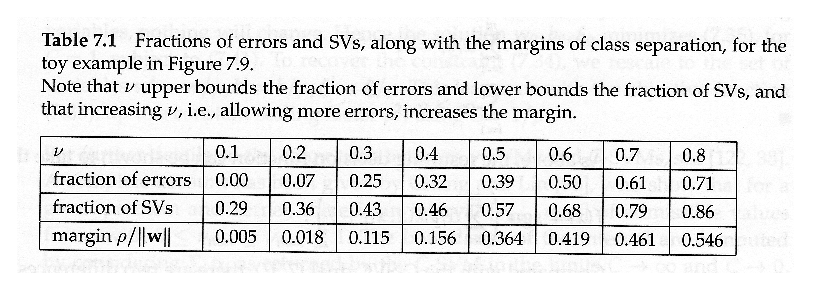
\includegraphics[height=30mm]{images/nu-svc-table.eps}
\end{center}

\vspace{.5in}
{\footnotesize (source: "Learning with Kernels", Sch\"olkopf and Smola, MIT, 2002) }

\es

\bs{$\nu$-SVR}
In $\nu$-SVR we want to have our $\varepsilon$ automatically computed.  This gives rise to the following primal optimization problem
\[
\min_{\ol{w},\ol{\xi},\ol{\xi}',\varepsilon,b} \phi(\ol{w},\ol{\xi},\ol{\xi}',\varepsilon,b) = \frac{1}{2}\ol{w}\bullet\ol{w} +C \cdot \left ({\color{red}\nu\varepsilon} + \frac{1}{n}\sum_{i=1}^n (\xi_i + \xi'_i) \right )
\]
\[
\begin{array}{rl}
\mbox{subject to} &(\ol{w}\bullet\ol{x}_i - b) -  y_i \le \varepsilon +\xi'_i\\
& y_i - (\ol{w}\bullet\ol{x}_i - b)\le \varepsilon +\xi_i\\
& \xi_i \ge 0\\
& \xi_i^* \ge 0\\
& \varepsilon \ge 0
\end{array}
\]
Notice that here the term $\nu\varepsilon$ determines how much the size of the $\varepsilon$ tube contributes to the optimization problem.
\es


\bs{Dual $\nu$-SVR}
{\small
This gives rise to the dual,
\fframe{
\[
\max_{\ol{\alpha},\ol{\alpha}'}  \phi'(\ol{\alpha},\ol{\alpha}') = 
  \max_{\ol{\alpha},\ol{\alpha}'}  
  \sum_{i=1}^l (\alpha_i - \alpha_i')y_i
  - \frac{1}{2}\sum_{i=1}^l \sum_{j=1}^l (\alpha_i - \alpha'_i)(\alpha_j - \alpha'_j) k(\ol{x}_i,\ol{x}_j)
\]
subject to the constraints,
\begin{eqnarray*}
&&\sum_{i=1}^l (\alpha_i - \alpha'_i) = 0 \\
&&\sum_{i=1}^l (\alpha'_i + \alpha_i) \le C\cdot\nu \\
&&C/l \ge \alpha_i,\alpha'_i  \ge 0,  i = 1,\ldots,l
\end{eqnarray*}
}
Our model is,
\[
\model{f}(\ol{x}) = \sum_{i = 1}^l (\alpha_i - \alpha'_i) k(\ol{x}_i, \ol{x}) - b.
\]


}
\es

\bs{$\nu$-SVR}
\begin{center}
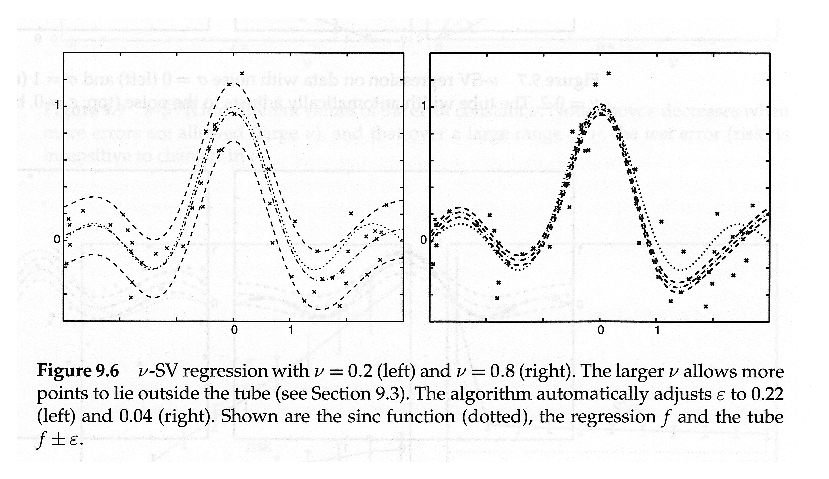
\includegraphics[height=60mm]{images/nu-svr.eps}
\end{center}
\es
\end{document}
%%%%%%%%%%%%%%%%%%%%%%%%%%% end of template1.tex %%%%%%%%%%%%%%%%%%%%%%%%%%%%%%%%

